

\section{Arquitecturas de Sistemas Operativos}
\subsection{Arquitectura Monolítica}
El sistema operativo monolítico es un sistema operativo muy simple donde el núcleo controla directamente la gestión de dispositivos, memoria, archivos y procesos. Todos los recursos del sistema son accesibles al núcleo. En los sistemas monolíticos, cada componente del sistema operativo está contenido dentro del núcleo.\\
En una arquitectura monolítica, el núcleo del sistema operativo está diseñado para proporcionar todos los servicios del sistema operativo, incluyendo la gestión de memoria, la programación de procesos, los controladores de dispositivos y los sistemas de archivos, en un único y gran binario. Esto significa que todo el código se ejecuta en el espacio del núcleo, sin separación entre los procesos del núcleo y los del usuario \citep{geeks_monolithic}.


\begin{figure}[H]
    \centering
    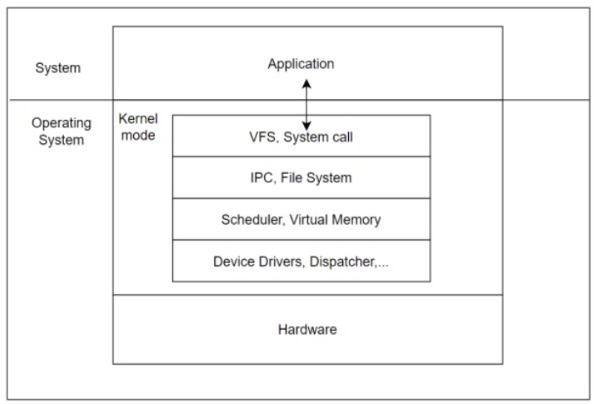
\includegraphics[width=0.7\textwidth]{figures/monolitica.jpeg}
    \caption[Sistema operativo basado en kernel monolítico]%
            {Sistema operativo basado en kernel monolítico \citep{harshvardhan2023kernels}}
    \label{fig:arquitectura_monolitica}
\end{figure}

\subsection{Arquitectura en Microkernel}
Un microkernel es un enfoque para diseñar un sistema operativo (SO). El microkernel proporciona servicios fundamentales para su funcionamiento, como la gestión básica de memoria, la programación de tareas.El microkernel es un tipo de sistema operativo que proporciona servicios básicos.\\
como los controladores de dispositivos y los sistemas de archivos, son gestionados por procesos a nivel de usuario. El proceso a nivel de usuario se comunica con el microkernel mediante el paso de mensajes. Esta forma de gestionar el proceso hace que los microkernels sean más modulares y flexibles que los kernels monolíticos tradicionales \citep{geeks_microkernel}.


\begin{figure}[H]
    \centering
    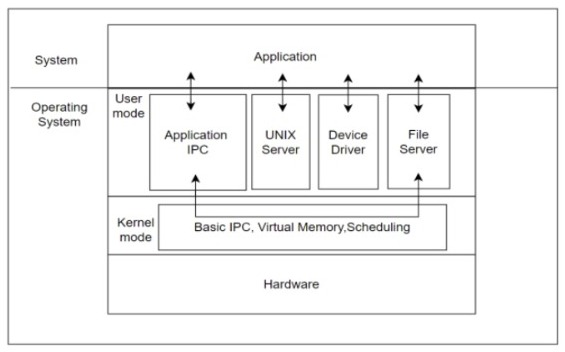
\includegraphics[width=0.7\textwidth]{figures/microkernel.jpeg}
    \caption[Sistema operativo basado en microkernel]%
            {Sistema operativo basado en microkernel \citep{harshvardhan2023kernels}}
    \label{fig:arquitectura_microkernel}
\end{figure}

\subsection{Arquitectura Hibrida}
Un núcleo híbrido es una arquitectura de núcleo basada en la combinación de aspectos de las arquitecturas de micronúcleo y núcleo monolítico utilizadas en sistemas operativos .\\
La idea de esta categoría es tener una estructura de kernel similar a la de un microkernel, pero implementada en términos de un kernel monolítico. A diferencia de un microkernel, todos (o casi todos) los servicios del sistema operativo se encuentran en el espacio del kernel . Si bien no hay sobrecarga de rendimiento para el paso de mensajes ni el cambio de contexto entre el kernel y el modo de usuario, como en los kernels monolíticos , no hay ventajas de rendimiento al tener servicios en el espacio de usuario , como en los microkernels \citep{ms_hybrid_kernel}.
\begin{figure}[H]
    \centering
    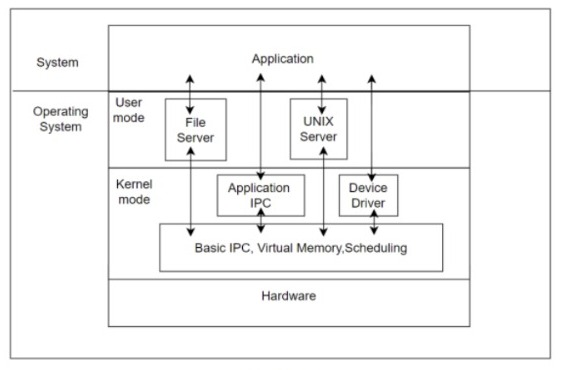
\includegraphics[width=0.7\textwidth]{figures/hibridokernel.jpeg}
    \caption[Sistema operativo basado en kernel híbrido]%
            {Sistema operativo basado en kernel híbrido \citep{harshvardhan2023kernels}}
    \label{fig:arquitectura_kernel_hibrido}
\end{figure}


\subsection{Arquitectura en Exokernel}
Exokernel es un sistema operativo desarrollado por el Instituto Tecnológico de Massachusetts (MIT) con el concepto de poner la aplicación bajo control. Los sistemas operativos Exokernel buscan proporcionar gestión de recursos de hardware a nivel de aplicación. La arquitectura de este sistema operativo está diseñada para separar la protección de recursos de la gestión, facilitando así la personalización específica de cada aplicación\citep{keetmalin2017exokernel}.




\begin{figure}[H]
    \centering
    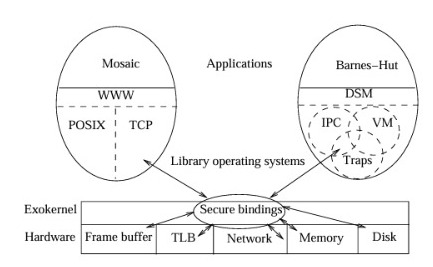
\includegraphics[width=0.7\textwidth]{figures/hexokernel.jpeg}
    \caption[Sistema operativo basado en exokernel]%
            {Sistema operativo basado en exokernel \citep{exokernel1995}}
    \label{fig:arquitectura_kernel_exokernel}
\end{figure}



\subsection{Comparacion entre arquitecturas de Sistemas Operativos}

\begin{muntab}{|c|p{5cm}|p{5cm}|}
  {comparacion_kernel}
  {Comparación de arquitecturas de SO basado mayormente en \citep{harshvardhan2023kernels}}
\hline
\textbf{Arquitectura} & \textbf{Ventajas} & \textbf{Desventajas} \\
\hline
Monolítica & Alto rendimiento, simple en diseño inicial & Difícil de mantener, poco modular \\
\hline
Microkernel & Modularidad, mayor seguridad & Mayor sobrecarga de comunicación \\
\hline
Hibrida & Combina rendimiento y modularidad & Complejidad de implementacion \\
\hline
Exokernel & Máxima flexibilidad y control & Muy complejo, poco usado en producción \\
\hline
\end{muntab}
